% !TEX root = slides.tex
%==================================================================================
\begin{frame}[t]
\label{bayespc}
\frametitle{Bayesian inference of PC surrogate: \small{high-d, low-data regime}}

\vspace*{-2mm}
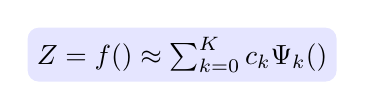
\begin{tikzpicture} \node [rounded corners,fill=blue!10] {
$Z =f(\vxi) \approx \sum_{k=0}^{K} c_k \Psi_k(\vxi)$
};
\end{tikzpicture}\\
\medskip
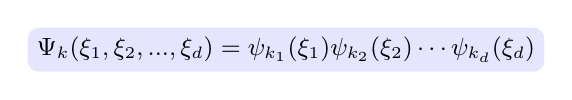
\begin{tikzpicture} \node [rounded corners,fill=blue!10] {
\small
$\Psi_k(\xi_1,\xi_2,...,\xi_d)=\psi_{k_1}(\xi_1) \psi_{k_2}(\xi_2) \cdots \psi_{k_d}(\xi_d) $
};
\end{tikzpicture}
%$\underbrace{P(\vc|\DD)}_{\color{blue}\textrm{Posterior}\color{black}}\propto \underbrace{P(\DD|\vc)}_{\color{blue}\textrm{Likelihood}\color{black}} \underbrace{P(\vc)}_{\color{blue}\textrm{Prior}\color{black}}$

%\only<1>{
%\small{
%\bri
%\item \underline{Data} consists of  \emph{training runs} \[ \DD\equiv\{(\vxi_i, u_i)\}_{i=1}^N \]
%\item \underline{Likelihood} with a gaussian noise model with $\sigma^2$ fixed or inferred,
%\ben
%L(\vc)=P(\DD|\vc)=\left(\frac{1}{\sigma\sqrt{2\pi}}\right)^N \prod_{i=1}^N \exp\left(-\frac{(u_i-g_\vc(\vxi))^2}{2\sigma^2}\right)
%\een
%
%\item \underline{Prior} on $\vc$ is chosen to be conjugate, uniform or gaussian.
%\vspace*{1mm}
%\item \underline{Posterior} is a \emph{multivariate normal} \[\vc\quad\in\quad{\cal MVN}(\vmu,\vSigma)\]
%\item The (uncertain) surrogate is \emph{a Gaussian process}
%\[\sum_{k=0}^{K-1} c_k \Psi_k(\vxi)=\vPsi(\vxi)^T \vc \quad\in\quad \GP(\vPsi(\vxi)^T \vmu, \vPsi(\vxi)\vSigma\vPsi(\vx')^T )  \]
%
%\eri
%}
%}
\vspace*{-6mm}

\large{
\vspace*{1cm}
\only<1->{
\bri
\item Issues:
\vspace*{0.5cm}
\bbi
\item \parbox{0.4\textwidth}{how to properly choose the basis set?}\hfill \hspace*{5.5cm}\parbox{0.6\textwidth}{\vspace*{0.5cm}\smash{
\includegraphics<1>[width=1.8in]{bcsclm/mi_td.eps}
\includegraphics<2>[width=1.8in]{bcsclm/mi_tp.eps}
\includegraphics<3>[width=1.8in]{bcsclm/mi_hc.eps}
\includegraphics<4>[width=1.8in]{bcsclm/mi_hdmr.eps}
\includegraphics<5>[width=1.8in]{bcsclm/mi_lq05.eps}
}}
\item need to work in underdetermined regime $N<K$: fewer data than bases (d.o.f.)
\ebi
\vspace*{0.8cm}
\item Discover the underlying low-d structure in the model
\vspace*{0.3cm}
\bbi
\item get help from the machine learning community
\vspace*{0.3cm}
\ebi
\eri
}
}
\end{frame}
%==================================================================================
